\documentclass[11pt]{article}

\usepackage[font=footnotesize]{caption}
\usepackage{float}
\usepackage{epsf}
\usepackage{epsfig}
\usepackage{subfigure}
\usepackage{latexsym}
\usepackage{booktabs}
\usepackage{graphicx}
\usepackage[table,xcdraw]{xcolor}
\usepackage{color, colortbl}
\usepackage{wrapfig}
\usepackage{multirow}
\usepackage{tabularx}
\usepackage{hyperref}
\usepackage{xcolor}
\usepackage{mdwlist}
\usepackage{pdfpages} 
\usepackage{tabto}  



\usepackage{amsmath, amsfonts, amssymb}
\usepackage[hmargin=1in,vmargin=1.2in]{geometry}
\usepackage{url}
\usepackage{multirow}
\usepackage[bottom]{footmisc}
\usepackage{afterpage}
\usepackage{eurosym}
\usepackage{enumitem}
\usepackage{soul}
% *******************************************
\usepackage{lineno}
\usepackage{setspace}
% *******************************************

\interfootnotelinepenalty=80 
\floatingpenalty=0\relax
\widowpenalty=1000
\clubpenalty=1000


\def\proj{{\textbf{FRESNEL\ }}}
\def\proje{{\textbf{FRESNEL}}}
\def\met{{\textbf{METEOR\ }}}
\def\mete{{\textbf{METEOR}}}
\def\naz{{Nazar\'{e}\ }}
\def\naze{{Nazar\'{e}}}

\setlength{\parskip}{0pt}
\setlength{\parsep}{0pt}
\setlength{\headsep}{0pt}
\setlength{\topskip}{0pt}
\setlength{\topmargin}{0pt}
\setlength{\topsep}{0pt}
\setlength{\partopsep}{0pt}

\newtheorem{definition}{Definition}
\newcommand{\hide}[1]{}
\newcommand{\kcomment}[1]{{\color{red}{KR: #1}}}
\newcommand{\rmcomment}[1]{{\color{blue}{RM: #1}}}
\newcommand{\com}[1]{{\color{blue}{#1}}}
\newcommand{\hcom}[1]{{\color{white}{#1}}}
\newcommand{\lc}[1]{\textcolor{blue}{#1}}

\newcounter{quotenumber}

% \newenvironment{numquote}{%
%     \begin{enumerate}%
%      \setcounter{enumi}{\value{quotenumber}}%
%      \color{darkgray}
%     \item \begin{quote}%
% }{%
%     \end{quote}%
%     \setcounter{quotenumber}{\value{enumi}}
%     \end{enumerate}%
% }%

% \makeatletter
% \def\myitem{%
%    \@ifnextchar[ \@myitem{\@noitemargtrue\@myitem[\@itemlabel]}}
% \def\@myitem[#1]{\item[#1]\mbox{}}
% \makeatother



% \newcommand\blankpage{%
%     \null
%     \thispagestyle{empty}%
%     \addtocounter{page}{-1}%
%     \newpage}

\setcounter{secnumdepth}{1} 

\let\oldthebibliography\thebibliography
\let\endoldthebibliography\endthebibliography
\renewenvironment{thebibliography}[1]{
  \begin{oldthebibliography}{#1}
    \setlength{\itemsep}{0em}
    \setlength{\parskip}{0em}
}
{
  \end{oldthebibliography}
}
% \linespread{0.98}
\parskip 0.1cm


\title{On Model-Driven Ocean Exploration}

\author{
Renato Mendes\textsuperscript{1,2,3,*},
Lucrezia Bernacchi \textsuperscript{1},
Leonardo Azevedo \textsuperscript{},
Ana F. Duarte \textsuperscript{},\\
Marina Cunha \textsuperscript{},
Clara Rodrigues \textsuperscript{},
João Borges de Sousa \textsuperscript{1,3},
João Vitorino \textsuperscript{},\\
Ajit Subramaniam \textsuperscript{},
Kanna Rajan \textsuperscript{}
\\
\\
\textsuperscript{1}{\scriptsize Laboratório de Sistemas e Tecnologia Subaquática (LSTS), Faculdade de Engenharia da Universidade do Porto, Portugal}\\
\textsuperscript{2}{\scriptsize +ATLANTIC CoLAB, Lisboa, Portugal}\\
\textsuperscript{3}{\scriptsize Laboratório Associado de Energia, Transportes e Aeronáutica (LAETA), Porto, Portugal}\\
\textsuperscript{1}{\scriptsize Universidade de Aveiro, Portugal}\\
\textsuperscript{1}{\scriptsize Lamont-Doherty Earth Observatory, Columbia University, New York}\\
\textsuperscript{1}{\scriptsize Instituto Hidrogr{\'a}fico Lisboa, Portugal}\\
\textsuperscript{1}{\scriptsize RAND Corporation, Washington D.C \& Faculdade de Engenharia da Universidade do Porto, Portugal}\\
\textsuperscript{*}\texttt{{\scriptsize renato.mendes@colabatlantic.com}}
}
\date{} 
\begin{document}

% \setcounter{secnumdepth}{2} 
% \vspace{+0.5cm}

\maketitle
\section{Introduction}
\label{sec:intro}

The coastal ocean, the marine areaS extending from the coastline to
the continental slope, encompassing the continental shelf, constitutes
one of the most dynamic and complex regions of the ocean. These areas
are characterized by highly variable forcing mechanisms, intricate
topographies, and coastline geometries. They are forced by a wide
range of physical and biogeochemical processes which occur across
diverse spatial and temporal scales. They are among the most
productive and economically significant areas of the world’s oceans,
benefiting from terrestrial inputs via river discharges and nutrient
renewal driven by upwelling processes. As a result and in part,
coastal areas concentrate a great proportion of human maritime
activities, from fisheries and offshore aquaculture to renewable
energy exploitation. Moreover, the coastal ocean acts as an interface
between deep-ocean processes and coastal environment, modulating how
large-scale phenomena — such as climate-driven changes or extreme
weather events — impact coastal populations. It also regulates, for
example, how anthropogenic influences originating on land are
redistributed and affect marine ecosystems \cite{greene25}.

The complex interplay between physical, chemical, and biological
processes in the coastal ocean can rapidly amplify or modulate the
impacts of extreme events such as storms, flooding, or pollution
incidents. Furthermore, the coastal ocean serves as a key interface
where large-scale oceanic and atmospheric changes manifest their
consequences for coastal ecosystems. Accurately forecasting the state
of the coastal ocean is therefore essential not only for safeguarding
environmental and economic interests, but also for enhancing
resilience to climate variability, natural hazards, and human-induced
pressures.  Achieving this, however, remains a major scientific and
technological challenge, given the high variability, rapid dynamics,
and observational constraints inherent to these regions.

Ocean models have become essential tools for predicting the ocean
state and underpin a wide range of societal applications, from climate
forecasting to pollution monitoring and resource management. However,
these models are inherently imperfect representations of complex
reality. Data assimilation techniques — where observational data are
integrated into models — play a critical role in correcting or
adjusting model errors and improving their forecasting
capabilities. Yet, the success of data assimilation depends heavily on
the availability, quality, and relevance of observations.

Observations of the ocean are obtained through multiple sources.
Satellite remote sensing offers extensive spatial coverage but is
limited to surface measurements with usually low spatial resolution
and often compromised by atmospheric conditions. In situ observations,
whether from ships, moorings, or drifting platforms, provide higher
accuracy but suffer from limited spatial and temporal coverage, high
operational costs, and logistical constraints — particularly high in
coastal regions. Recent technological advances have enabled the use of
autonomous underwater vehicles (AUVs) and other robotic platforms,
offering flexible, mobile, and increasingly autonomous means of
sampling ocean properties with high spatiotemporal resolution and low
logistic footprint
\cite{das10,das11b,olaya12,graham12,jdas13,das15,sousa16,fossum18,fossum19b}.

However, even with these new tools, efficiently gathering data at the
right spatial and temporal scales remains a complex challenge. AUVs
are constrained by endurance, communication bandwidth, and operational
risks such as vessel traffic, high currents and bathymetry. In
addition, the ocean itself remains highly dynamic with key processes
often evolving faster than traditional sampling strategies can
capture. This opens the door to adaptive sampling strategies, where
observation efforts are guided by model outputs and uncertainty
estimates to maximize the relevance of collected data. Adaptive
sampling \cite{BinZhang07,Singh09,smith14,fossum19} represents a
fundamental shift: instead of executing pre-planned missions,
autonomous vehicles dynamically prioritize areas for observation.

One approach that we articulate here is combining model predictions
with adaptive AUV sampling. Doing so combines predicted model
uncertainties in comparison with prior data assimilation process with
availabe obervations. Model forecasts identify where uncertainty is
highest or where new observations are expected to have the greatest
impact in reducing forecast errors. Vehicles are then directed to
sample these areas, and their data are in turn assimilated back into
the models, generating improved forecasts for subsequent adaptive
planning as a virtuous cycle. Doing so closes a critical feedback loop
between models and observations; model prediction generates a forecast
and associated uncertainty field while adaptive sampling targets areas
of maximum predicted uncertainty. Data assimilation from these high
uncertainty regions are then incorporated into the model such that new
predictions benefit from improved in-situ data, closing the loop.
Such a \textit{data cycle} approach promises to significantly enhance
the skill of ocean forecasts, especially in the complex coastal
environment where processes occur over a wide range of scales and
where human and environmental stakes are high. It also has the
potential to improve operational efficiency by optimizing the
deployment of costly and resource-constrained observational assets. 
WE MAY WANT TO EXPLAIN THAT THIS CAN ONLY BE DONE WITH AUVS AND AT A MODERATE COST IN COMPARISON TO TRADITIONAL SAMPLING METHODS


IT MAY ALSO BE A GOOD IDEA TO HAVE A SHORT PARAGRAPH OM INNOVATION CLAIMS: something like

This has been done before, but we innovate in several aspects: 
\begin{itemize}
    \item Near-real time data visualization enable real.time response by operators..
    \item Simultaneous deployments in geographically separate subareas in the area of operations.
    \item Coordination also included risk minimizing considerations. This enabled operations in tight time intervals to collect data where it was needed taking advantage of openings provided by trawlers between consective legs.
    \item Parameterized framework enabling fine tuning of the overall approach. 
    \item Dense grid of observations.
    \item The sampling algorithm is not based only on position, but on error distributions and closed tours to maximize area coverage and utilization of the auvs.
    \end{itemize}

WHAT DO YOU THINK?

\begin{figure}[!]
  \centering
  \includegraphics[scale=0.5]{fig/ensemble-2.jpg}
  \caption{\proj demonstrates the value of integrating ocean models
    with adaptive robotic vehicles in the coastal ocean, to increase
    model skill while increasing model accuracy and prediction within
    a tight control loop.}
  \label{fig:block-diag}
\end{figure}



In this study, we address the challenge of such loop closure by
implementing and evaluating a complete data cycle — from model
prediction, to uncertainty projection, to adaptive sampling and data
assimilation — in a coastal ocean environment. The work was conducted
within the framework of \proj (\textbf{F}ield expe\textbf{R}iments for
mod\textbf{E}ling, a\textbf{S}similatio\textbf{N} and
adaptiv\textbf{E} samp\textbf{L}ing), a project specifically designed
to explore and test model-driven robotic exploration strategies. \proj
provided the experimental setting and operational assets to
demonstrate how model-based uncertainty fields can drive adaptive
sampling missions aimed at improving ocean model predictive skills to
enhance ocean forecasts in highly dynamic coastal environments
(Fig. \ref{fig:block-diag}). The experimental results obtained within
\proj serve to illustrate and validate the proposed approach,
highlighting the practical benefits and challenges of real-world
adaptive ocean exploration. Furthermore, we demonstrate that this
sampling robotic system offers unprecedented capabilities for ocean
studies by providing samples in close to real-time and enabling
scientists to adaptively re-task AUVs within minutes if some
interesting feature is detected.


\section{Study Area}
\label{sec:study-area}

\begin{figure}[!t]
  \vspace{-0.5cm}
  \centering
  \subfigure[Map of Portugal and the study area highlighted with the
  red rectangle.]{\label{fig:po-map}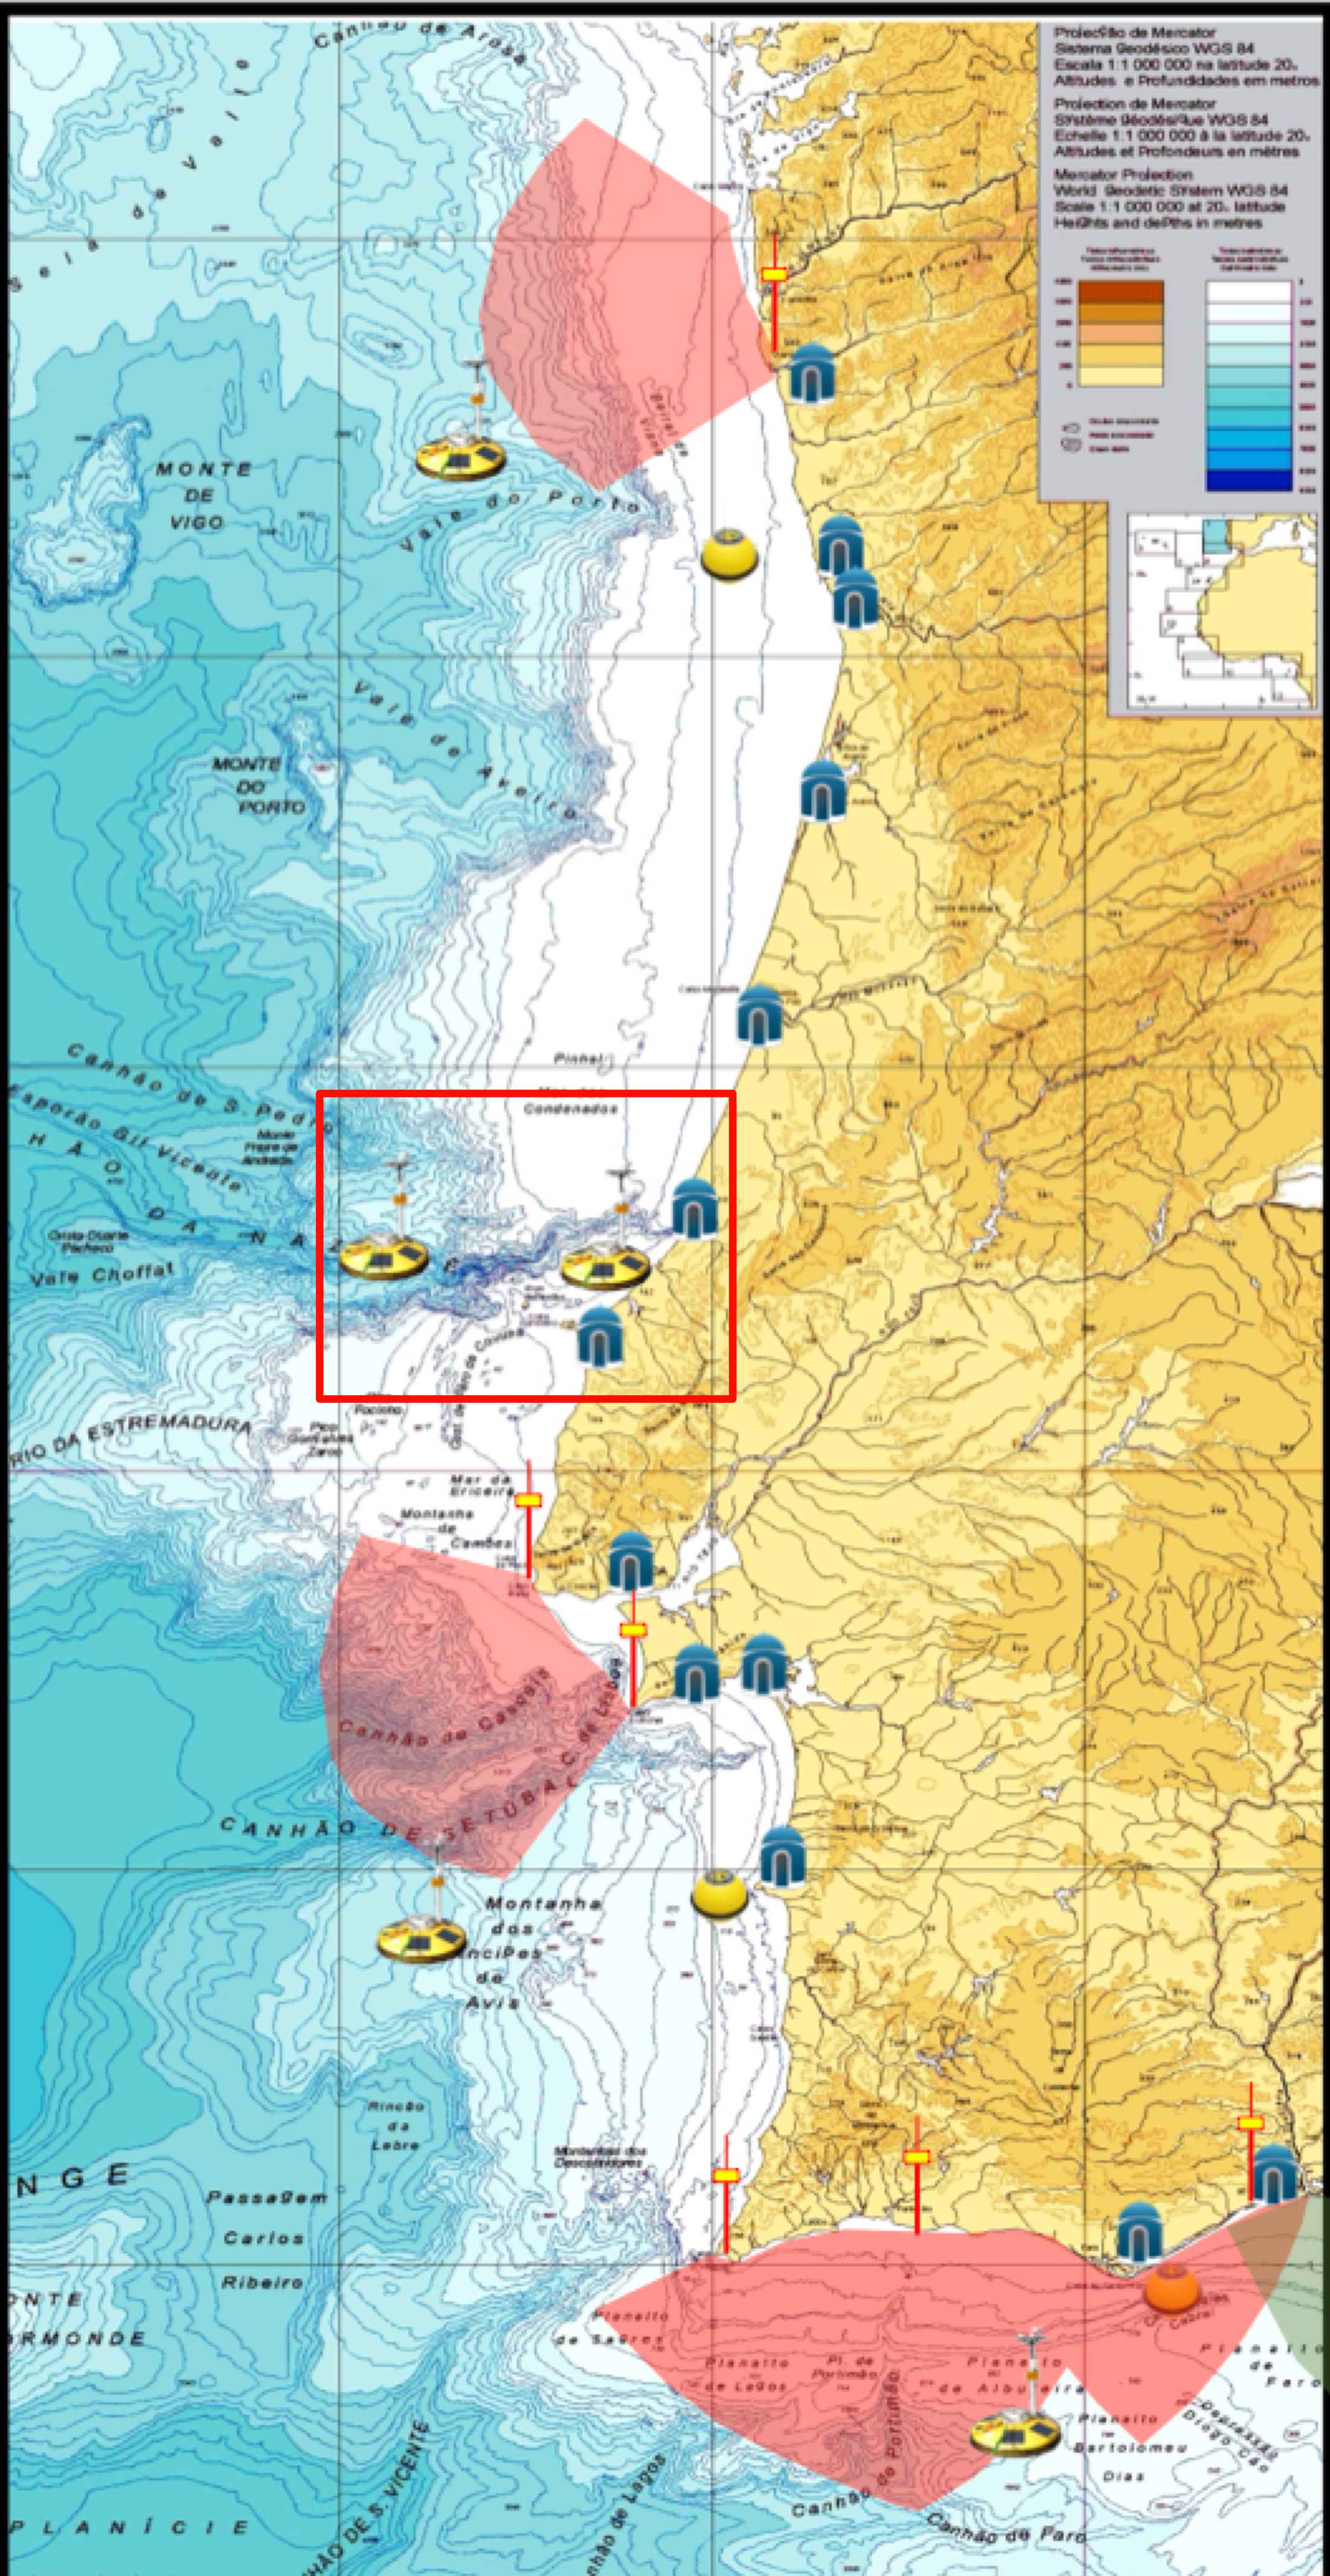
\includegraphics[scale=0.2]{fig/po-map.png}}
  \hspace{+0.3cm}
  \subfigure[Bathymetry showing the \naz canyon-Berlengas area
  and its environment.]{\label{fig:domain}\includegraphics[scale=0.19]{fig/area_ripples.png}}
  \caption{\subref{fig:po-map} \& \subref{fig:domain} show detailed
    views of the study area for \proj off the coast of mainland
    Portugal. The \naz Canyon is a significant feature of this area
    and a driver for the bio-geophysics of the domain
    \cite{tyler2009europe}.}
  \label{fig:studyarea-1}
\end{figure}


% \begin{wrapfigure}{!h}{2.75in}
%   \centering
%  \includegraphics[scale=0.2]{fig/data_cycle.png}
%  \caption{\proje's approach attempts to close the
%    \emph{sample-assimilate-predict-direct} loop using data obtained
%    from robotic vehicles assimilated into a model which generates a
%    prediction which in turn is used to inform the sampling strategy of
%    the robotic vehicles to reduce model uncertainty.}
%   \label{fig:loop-closure} 
% \end{wrapfigure}

The study was conducted in the coastal ocean off central Portugal,
focusing on the region influenced by the \naz Canyon (39.2$^{\circ}$
- 39.9$^{\circ}$N) (Fig. \ref{fig:studyarea-1}) during fall of
2024. While the experiment considered the measurable impact of model-driven robotic sampling to both the bio-geochemistry of the canyon
region, this manuscript is focused on the implications of closing the
\emph{sample-assimilate-predict-direct} loop closure.
% (Fig. \ref{fig:loop-closure}).

Implementing such a closed-loop system in a dynamic coastal environment presents substantial challenges. These included the need for high-resolution numerical models capable of rapidly generating uncertainty projections, robust algorithms for exploration under a range of constraints, reliable communication links for mission updates, and assimilation frameworks that integrate heterogeneous real-time data streams. Furthermore, marine operations face logistical risks and communication limitations — such as low bandwidth, intermittent connectivity, and unpredictable weather — that further constrain the execution of adaptive sampling missions.

The \naz area features pronounced topographic contrasts: the
transition from the wide Estremadura Plateau to the narrower northern shelf, the long and narrow \naz submarine canyon that incises the
shelf and extends more than 200km offshore, and the Berlengas
archipelago, a UNESCO Biosphere Reserve with high ecological
value. These features contribute to enhanced biological productivity
and biodiversity, and strongly modulate physical and biogeochemical
processes in the region.

Freshwater inputs from major rivers, such as the Tagus, have only a
limited direct impact on the area. In contrast, smaller rivers and the
\'{O}bidos lagoon can episodically deliver low-salinity, nutrient-rich
plumes to the shelf. Circulation is driven by seasonal wind
forcing linked with the Azores High, with persistent
upwelling-favorable northerly winds in summer and frequent downwelling
episodes in winter under southerly winds. The interplay between canyon
topography, shelf circulation, and atmospheric forcing generates
complex mesoscale dynamics, intensified tidal currents, and internal
wave activity that promote strong vertical mixing and cross-shelf
exchanges \cite{martins10,quaresma07}.

The combination of sharp bathymetric gradients, variable forcing, and
rich physical–biogeochemical interactions makes the \naz Canyon region
an ideal natural laboratory to test adaptive observation
strategies. In particular, its dynamic environment posed both
opportunities and challenges for the \proj experiment, providing a
representative coastal setting in which to evaluate how model-based
uncertainty projections can guide adaptive sampling and assimilation
to improve ocean model predictive skill.


\section{Methods}
% max 3000 words

Our methodology is based on the implementation of a complete data cycle to enhance model predictions in a coastal ocean domain through adaptive sampling and data assimilation. The approach consists of three fundamental steps, executed iteratively on a daily basis:

\begin{enumerate}
    \item \textbf{Model Forecast and Uncertainty Projection}:  
    A numerical ocean model provides a daily one-step forecast $\hat{\theta}(k+1, x, y)$ of a target oceanic variable $\theta$, along with an associated uncertainty field $\sigma_{\hat{\theta}}(k+1, x, y)$, where $k$ represents the current day and $(x, y)$ denote the geographical coordinates. These outputs are organized into discrete spatial maps, $M_{\hat{\theta}}(x, y)$ and $M_{\sigma_{\hat{\theta}}}(x, y)$, representing, respectively, the predicted state and its uncertainty over a predefined grid covering the study area.
    
    \item \textbf{Adaptive Sampling Planning}:  
    Using the uncertainty map $M_{\sigma_{\hat{\theta}}}(x, y)$ as input, an adaptive sampling algorithm determines the set of trajectories for a fleet of $N$ Autonomous Underwater Vehicles (AUVs) for the next operational cycle. The goal is to maximize the accumulated uncertainty sampled along the vehicle paths, while satisfying vehicle-specific constraints such as maximum endurance, operational limits, and navigation feasibility. The planned trajectories are transmitted to the vehicles for execution.

    \item \textbf{Data Collection and Assimilation}:  
    Throughout the operational period, each AUV collects pointwise measurements of the target variable $\theta$ along its assigned path. After the mission is completed, the collected measurements are assimilated into the numerical model using an appropriate data assimilation scheme. This updated model state serves as the new initial condition for the next forecasting cycle, closing the loop.
\end{enumerate}



\subsection{Available Models}
\subsection{Adaptive Sampling Algorithm}
\subsection{Available robotic systems and assets}

% The adaptive sampling problem is formulated as an optimization task aiming to maximize the expected information gain from the observations. Specifically, given the predicted uncertainty map and operational constraints (e.g., time, energy budget), the algorithm plans vehicle routes that prioritize areas of higher model uncertainty. The uncertainty along each candidate path is evaluated, and path planning strategies — such as greedy heuristics or combinatorial optimization techniques — are employed to allocate waypoints efficiently among the available AUVs.

\subsection{Operational Constraints and Practical Considerations}

% The practical implementation of the data cycle in a real-world marine environment introduces several constraints:

% \begin{itemize}
%     \item \textbf{Communication Limitations}:  
%     Low-bandwidth and intermittent communications at sea require that mission planning be sufficiently robust to accommodate long periods of autonomous operation without human intervention.
    
%     \item \textbf{Vehicle Constraints}:  
%     AUV endurance, payload limitations, navigation precision, and deployment risks all impose restrictions on the feasible operational space and mission duration.

%     \item \textbf{Computational Demands}:  
%     Real-time generation of uncertainty fields, optimization of paths, and assimilation of collected data must be performed within time windows compatible with daily operational cycles, often under constrained computational resources.

%     \item \textbf{Environmental Variability}:  
%     Fast-evolving coastal ocean dynamics can introduce discrepancies between forecasted and actual conditions, necessitating robust planning that accounts for forecast uncertainty and adaptivity.
% \end{itemize}

% This method was deployed and evaluated under the operational framework of the FRESNEL project, providing a real-world demonstration of the data cycle’s feasibility and benefits in complex coastal environments.


% Distinction Between Onboard and Offboard Predictions:
% \begin{itemize}
%     \item Onboard: Statistical prediction
%     \item Offboard: Numerical prediction
% \end{itemize}

% Rationale and Implementation (including a schematic figure):
% \begin{itemize}
%     \item Why this approach?
%     \item How was it executed?
% \end{itemize}

% Adaptive Sampling Strategy:
% \begin{itemize}
%     \item contraints
%     \item Algorithm used for real-time decision-making
%     \item Criteria for data collection optimization
% \end{itemize}

% Statistical Approach:
% \begin{itemize}
%     \item Techniques applied for uncertainty estimation
%     \item Integration with observational data
% \end{itemize}

%  Numerical Model (HOPS - Harvard Ocean Prediction System):
% \begin{itemize}
%     \item Model configuration and setup
%     \item Data assimilation methods
% \end{itemize}



\section{Results}
\textit{- Present your \textbf{findings} in a logical and coherent manner.}

\begin{itemize}
    \item Environmental context
    \item Results day-by-day
\end{itemize}

 
\textit{- Use \textbf{subheadings} to organize different experiments or analyses.}

\section{discussion}

\textit{- Interpret your results, discussing their \textbf{implications}, \textbf{limitations}, and how they compare to previous work.}

\textit{- This section should be \textbf{succinct} and may not contain subheadings.}



\bibliographystyle{IEEEtran}
\footnotesize{
  % \bibliography{ref,smedsrud,biblio}
  \bibliography{ref}
}
\end{document} 
